\section{\xxx Overview} \label{sec:overview}

Figure 2 shows \xxx's architecture. The replication logic is entirely 
implemented in qemu-kvm, a KVM tailored version of QEMU. It contains 
four main components: a \paxos consensus protocol for input coordination, 
an output checking protocol, a circular in-memory consensus log, and a 
guard process that handles checkpointing and recovering a server's process 
state and file system state.

% On receiving a packet, QEMU calls tap_send()
% On sending a packet, QEMU calls tap_receive()
% We maintain a packet queue to capture outgoing packets.

\begin{figure}[t]
% \vspace{.20in}
\centering
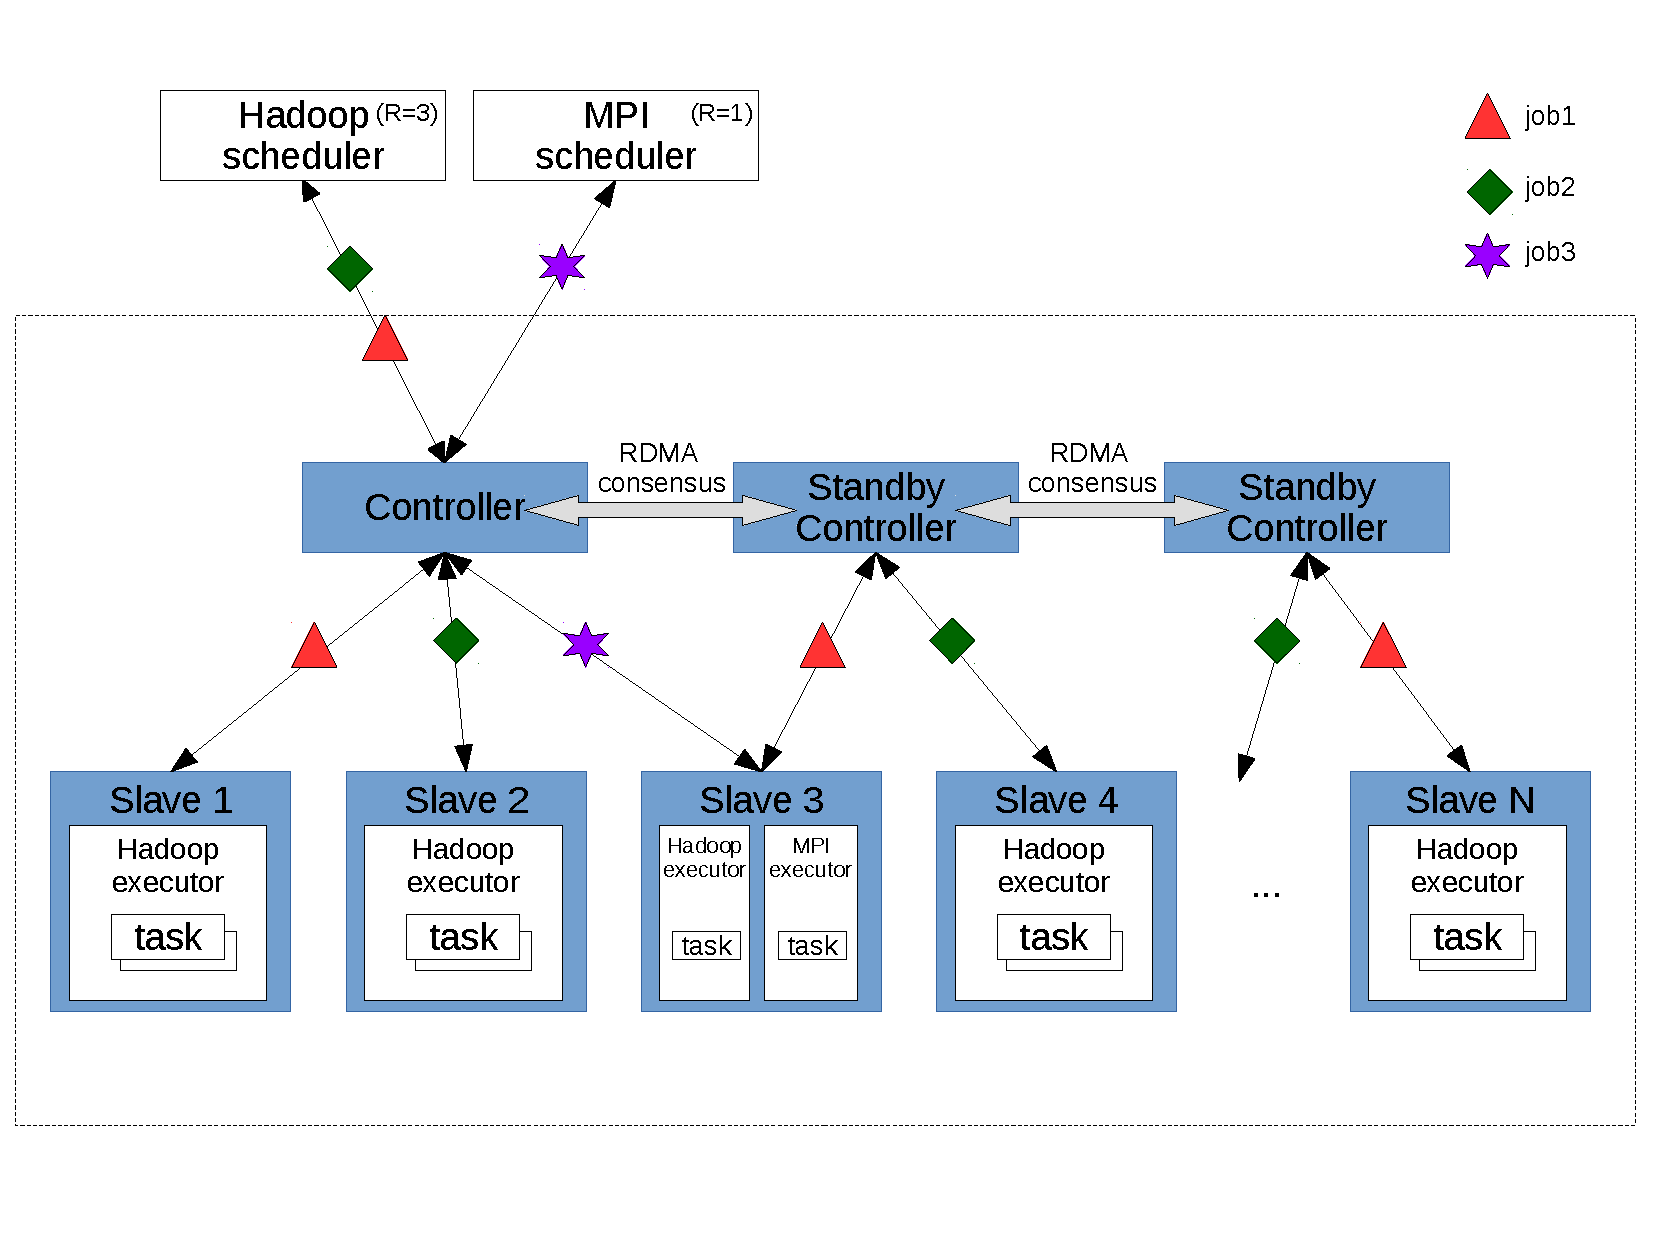
\includegraphics[width=.47\textwidth]{figures/arch}
\vspace{-.2in}
\caption{{\em The \xxx Architecture.}} \label{fig:arc}
\vspace{.05in}
\end{figure}
